\documentclass{altsu-report}
\linespread{1,5}
\title{Менеджер задач}
\author{А.\,В.~Лаптев}

\begin{document}
\setcounter{page}{3}
\tableofcontents

\chapter{Актуальность и востребованность разрабатываемого продукта}

В современном мире множество малых и средних компаний, которые занимаются разработкой различного рода программного обеспечения. В то время, как крупные компании давно и успешно используют для контроля и ведения разработки менеджеры задач, которые уже давно находятся на рынке и хорошо зарекомендовали себя, малые и средние компании и предприятия практически никогда не используют подобные технологии в своих проектах за счет их высокой стоимости и функционала, который для таких компаний может быть избыточными да и в целом менеджер задач может быть очень нагруженным с функциональной точки зрения, что требует временных затрат на обучение сотрудников.

Для подобных организаций имеет смысл иметь менеджер задач, который будет иметь базовый функционал, необходимый для ведения разработки и интуитивно-понятный интерфейс для взаимодействия с пользователем.

\chapter{Цель и задачи проекта и исполнители}

В рамках решения данной проблемы была поставлена следующая цель: разработка программного продукта для помощи в решении различных рабочих задач организации.

Для достижения поставленной цели было необходимо решить следующие задачи:

\begin{enumerate}
    \item Разработать простой и интуитивно понятный пользовательский интерфейс;
    \item Создать современный дизайн и использовать современные технологии в разработке;
    \item Создать продукт, который будет работать на ПК типовой комплектации со свободным выходом в Интернет;
    \item Реализовать запуск приложения без привязки к браузеру;
    \item Реализовать базовый функционал, которого будет достаточно для помощи в решении рабочих задач.
\end{enumerate}

Исполнителями данного проекта являются: Половинкин А.~Е. и Лаптев А.~В.

\chapter{Общие сведения о проделанной работе}

Ход выполнения работы был разделен на следующие этапы:

\begin{enumerate}
    \item Определение формата реализации (Web-приложение, Desktop-приложение, др.);
    \item Определение стека технологий, которые будут задействованы в разработке;
    \item Разработка backend;
    \item Разработка frontend;
    \item Проверка интеграции frontend и backend;
    \item Разработка дизайна Web-приложения;
    \item Тестирование готового продукта.
\end{enumerate}

На первом этапе необходимо было определиться с форматом реализации менеджера задач. В итоге был выбран формат Web-приложения, поскольку такой формат не требует места на накопителе, а также позволяет сразу же синхронизировать любые изменения в списке задач для пользователей.

Далее было необходимо определиться со стеком технологий, которые будут использованы для разработки. Готовое решение должно быть современным и отвечать текущим тенденциям в ...

По этим причинам были выбраны следующие технологии для использования во время разработки:

\begin{enumerate}
    \item В качестве фреймворка для RESTfull API разработки был выбран FastAPI. FastAPI —- это современный, быстрый (высокопроизводительный) веб-фреймворк для создания API используя Python 3.6+, в основе которого лежит стандартная аннотация типов Python.
    
    FastAPI активно использует декораторы, аннотации типов и интроспекцию кода, что позволяет уменьшить количество шаблонного кода в веб-приложении.

    Ключевые особенности FastAPI, которые повлияли на выбор данного фреймворка:
    
    \begin{enumerate}
        \item Скорость: Очень высокая производительность, на уровне NodeJS и Go (благодаря Starlette и Pydantic). Один из самых быстрых фреймворков Python;
        \item Быстрота разработки: Позволяет увеличить скорость разработки примерно на 200–300\%;
        \item Меньше ошибок: Сокращено примерно на 40\% количество ошибок, вызванных человеком (разработчиком). Этот и предыдущий пункт подтверждены лишь тестами внутренней команды разработчиков;
        \item Интуитивно понятный: Отличная поддержка редактора. Автозавершение везде. Меньше времени на отладку;
        \item Лёгкость: Разработан так, чтобы его было легко использовать и осваивать. Меньше времени на чтение документации;
        \item Краткость: Сведено к минимуму дублирование кода. Каждый объявленный параметр -- определяет несколько функций;
        \item Надежность: На выходе получается готовый к работе код. С автоматической интерактивной документацией;
        \item На основе стандартов: Основан на открытых стандартах API и полностью совместим с ними: OpenAPI (ранее известном как Swagger) и JSON Schema.
    \end{enumerate}

    \item В качестве СУБД был выбран PostgreSQL. PostgreSQL -- свободная объектно-реляционная система управления базами данных (СУБД).

    Сильными сторонами PostgreSQL считаются:
    
    \begin{enumerate}
        \item Высокопроизводительные и надёжные механизмы транзакций и репликации;
        \item Расширяемая система встроенных языков программирования: в стандартной поставке поддерживаются PL/pgSQL, PL/Perl, PL/Python и PL/Tcl;
        \item Дополнительно можно использовать PL/Java, PL/PHP, PL/Py, PL/R, PL/Ruby, PL/Scheme, PL/sh и PL/V8, а также имеется поддержка загрузки модулей расширения на языке C;
        \item Наследование;
        \item Возможность индексирования геометрических (в частности, географических) объектов и наличие базирующегося на ней расширения PostGIS;
        \item Встроенная поддержка слабоструктурированных данных в формате JSON с возможностью их индексации;
        \item Расширяемость (возможность создавать новые типы данных, типы индексов, языки программирования, модули расширения, подключать любые внешние источники данных).
    \end{enumerate}
    
    PostgreSQL допускает использование функций, возвращающих набор записей, который далее можно использовать так же, как и результат выполнения обычного запроса.
    
    PostgreSQL поддерживает одновременную модификацию БД несколькими пользователями с помощью механизма Multiversion Concurrency Control (MVCC). Благодаря этому соблюдаются требования ACID и практически отпадает нужда в блокировках чтения.

    \item Для создания пользовательских интерфейсов был выбран JavaScript-фреймворк с открытым исходным кодом -- Vue.js. Легко интегрируется в проекты с использованием других JavaScript-библиотек. Может функционировать как веб-фреймворк для разработки одностраничных приложений в реактивном стиле.

    Основные достоинства Vue.js:

    \begin{enumerate}
        \item Можно использовать только знания JavaScript и HTML;
        \item Возможно применение Typescript;
        \item В Vue.js реализуется шаблон MVVM;
        \item Vue.js предлагает возможность привязки данных на Javascript, так что вывод и ввод данных сопрягаются непосредственно с источником данных;
    \end{enumerate}
    
    Vuetify -- это библиотека пользовательского интерфейса, не требующая навыков дизайна, с красиво созданными вручную компонентами Vue.

    \item Проверка данных и управление настройками с использованием аннотаций типа Python -- для этих целей использовался Pydantic.

    Pydantic использует некоторые интересные новые языковые функции, а также:
    
    \begin{enumerate}
        \item Отлично работает с IDE/линтером/мозгом: Нет нового микроязыка определения схемы для изучения. Если программисту известно, как использовать подсказки типов Python, ему известно, как использовать pydantic . Структуры данных —- это просто экземпляры классов, которые определяются с помощью аннотаций типов, поэтому автодополнение, linting, mypy , IDE (особенно PyCharm ) должны правильно работать с проверенными данными;
        \item Двойное использование: Класс BaseSettings pydantic позволяет использовать pydantic как в контексте «проверить данные этого запроса», так и в контексте «загрузить настройки моей системы». Основные отличия заключаются в том, что системные настройки можно считывать из переменных среды, и часто требуются более сложные объекты, такие как DSN и объекты Python;
        \item Быстрый: Pydantic всегда серьезно относился к производительности, большая часть библиотеки скомпилирована с помощью cython, что дает ускорение ~ 50\%, обычно это так же быстро или даже быстрее, чем у большинства подобных библиотек;
        \item Проверка сложных структур: Использование рекурсивных пидантических моделей , typingстандартных типов (например List, Tuple, Dictи т. д.) и валидаторов позволяет четко и легко определять, проверять и анализировать сложные схемы данных;
        \item Расширяемый: Pydantic позволяет определять пользовательские типы данныхvalidator , или вы можете расширить проверку с помощью методов на модели, украшенной декоратором;
        \item Интеграция классов данных: Кроме того BaseModel, pydantic предоставляет dataclassдекоратор, который создает классы данных Python с анализом и проверкой входных данных.
    \end{enumerate}

    \item Для синхронизации объектов Python и записей реляционной базы данных была выбрана библиотека SQLAlchemy -- это программная библиотека на языке Python для работы с реляционными СУБД с применением технологии ORM. SQLAlchemy позволяет описывать структуры баз данных и способы взаимодействия с ними на языке Python без использования SQL.
    
    SQLAlchemy -- это набор инструментов Python SQL и Object Relational Mapper, который дает разработчикам приложений всю мощь и гибкость SQL.
    
    Работает back-end для баз данных: MySQL, PostgreSQL, SQLite, Oracle и других, между которыми можно переключаться изменением конфигурации.
    
    Основные возможности:
    
    \begin{enumerate}
        \item Использование ORM не является обязательным;    
        \item Устоявшаяся архитектура;
        \item Возможность использовать SQL, написанный вручную;    
        \item Поддержка транзакций;
        \item Создание запросов с использованием функций и выражений Python;
        \item Модульность и расширяемость;
        \item Дополнительная возможность раздельного определения объектного отображения и классов;
        \item Поддержка составных индексов;
        \item Поддержка отношений между классами, в том числе «один-ко-многим» и «многие-ко-многим»;
        \item Поддержка ссылающихся на себя объектов;
        \item Предварительная и последующая обработка данных (параметров запроса, результата) и другие.
    \end{enumerate}
    
    Использование SQLAlchemy для автоматической генерации SQL-кода имеет несколько преимуществ по сравнению с ручным написанием SQL:
    
    \begin{enumerate}
        \item Безопасность. Параметры запросов экранируются, что делает атаки типа внедрение SQL-кода маловероятными;
        \item Производительность. Повышается вероятность повторного использования запроса к серверу базы данных, что может позволить ему в некоторых случаях применить повторно план выполнения запроса;
        \item Переносимость. SQLAlchemy, при должном подходе, позволяет писать код на Python, совместимый с несколькими back-end СУБД. Несмотря на стандартизацию языка SQL, между базами данных имеются различия в его реализации, абстрагироваться от которых и помогает SQLAlchemy.
    \end{enumerate}
\end{enumerate}

После этого началась разработка backend части приложения. Backend решения представлен несколькими взаимодействующими контейнерами Docker. В одном контейнере развёрнута БД, где хранятся сами задачи и информация связанная с ними. В другом развернута API для работы с БД. 

\begin{figure}
    \centering
    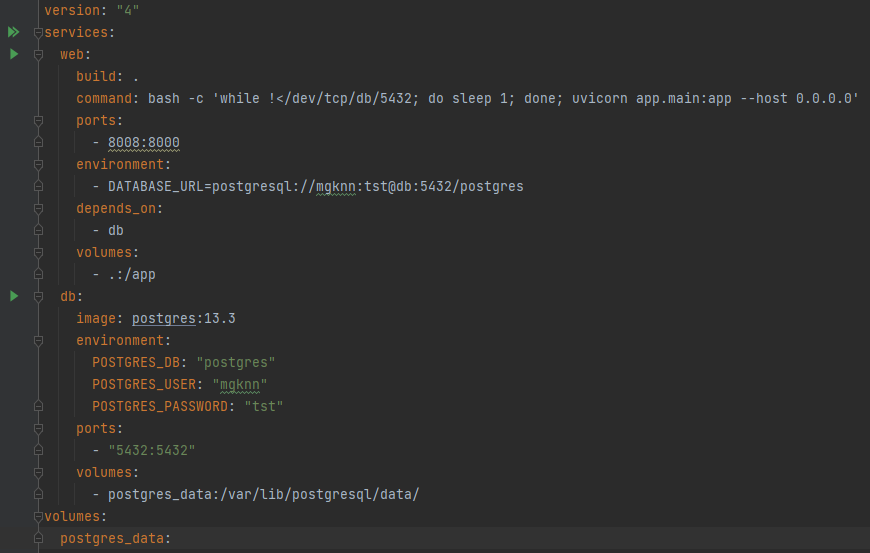
\includegraphics[scale=0.7]{docker.png}
    \caption{Файл Docker для запуска контейнеров.}
    \label{fig:enter-label}
\end{figure}

После того, как были реализованы frontend и backend. API отвечающая за взаимодействие web интерфейса и базы данных представляет из себя набор асинхронных методов. Каждый из методов выполняет свою функцию: от добавления новой задачи, до удалению уже существующей. При этом данные проходят проверку на соответствие типов, что исключает возможность занесения некорректных данных в таблицы базы данных.

\begin{figure}
    \centering
    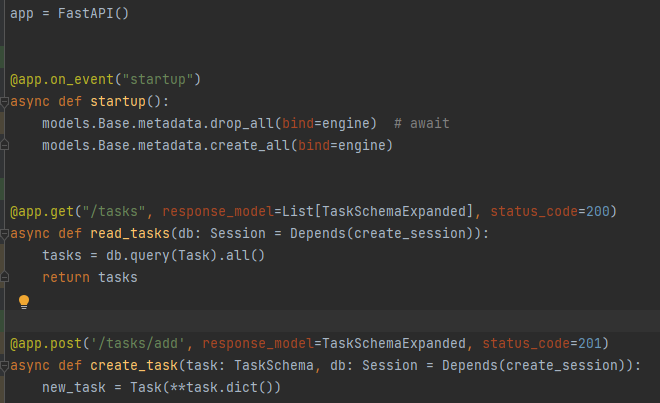
\includegraphics[scale=0.9]{api.png}
    \caption{API проекта.}
    \label{fig:enter-label}
\end{figure}

Frontend проекта разворачивается с помощью npm. Кнопки, таблицы и другие элементы разработанного веб интерфейса путем вызов методов API позволяют вести работу с задачами: добавлять, удалять, редактировать и т.д. Помимо функционала для frontend составляющей проекта был выработан и стиль, который применялся для всех элементов интерфейса. Была подобрана цветовая палитра, определено положение всех кнопок и областей, выбраны иконки. 

После завершения основной разработки было произведено ручное тестирование функционала всего приложения:

\begin{enumerate}
    \item Создание новой задачи;
    \item Редактирование существующей задачи;
    \item Удаление задачи;
    \item Изменение статуса задачи.
\end{enumerate}

Весь функционал отрабатывал стабильно и без ложных срабатываний, никаких багов в ходе тестирования найдено не было.

\chapter{Результаты проекта}

Конечный программный продукт представляет собой web-приложение --- менеджер задач, обладающий необходимым базовым функционалом для помощи в ведении разработки. В частности, он обеспечивает следующие возможности:

В качестве СУБД был выбран PostgreSQL. Работа с БД осуществляется из Python с помощью SQLAclhemy. С помощью этого инструмента при первичном запуске beckend'а происходит создание таблицы для наших будущих задач. Этим же инструментом, когда мы получаем соответствующие запросы, идет редактирование, удаление и создание задач.

У данного продукта есть свои сильные и слабые стороны.

К достоинствам можно отнести следующее:

\begin{enumerate}
    \item Использование быстрых и современных фреймворков и расширений к ним.
    \item Автоматизация ряда задач, которые включают в себя работу с БД.
    \item Простоту в использовании, за счет удобного интерфейса и навигации в нем.
    \item Малую потребность в ресурсах, поскольку данное решение не является перегруженным функционалом.
    \item Возможность расширения функционала.
\end{enumerate}

Программную реализацию этого механизма можно увидеть в приложении.

\begin{enumerate}
    \item Отслеживание текущих задач на главном экране с их валлидацией по времени --- более новые задачи добавляются в конец, толкая более старые вверх перечня, что обеспечивает меньшую путаницу и помогает держать в поле зрения задачи, которые требуют больше времени для решения;
    \item Создание новой задачи;
    \item Удаление (закрытие) задачи;
    \item Редактирование задачи.
\end{enumerate}

Менеджер задач работает на всех устройствах, включая смартфоны, и не имеет никаких проблем с масштабированием интерфейса под разные соотношения сторон и диагонали. Функционал также не зависит от выбранного устройства.

Ниже будет представлено более подробное описание каждого из них.

\section*{Главный экран}
\addcontentsline{toc}{section}{Главный экран}

Главный экран представляет собой минималистично оформленную страницу, на которой в заголовке обозначены две кнопки, с помощью которых можно обновить количество задач (динамического обновления пока что не присутствует) и создать новую задачу соответственно.

Ниже представлен перечень задач, в сортировке от более старой к более новой.

Для каждого статуса задачи предусмотрена разная сила подсветки. Предусмотрены следующие статусы:

\begin{enumerate}
    \item Задача создана;

    \item Задача в работе;

    \item Задача завершена.
\end{enumerate}

На рис. 1. показано то, как выглядит главный экран приложения при нескольких созданных активных и завершенных задачах.

\begin{figure}[!ht]
    \centering
    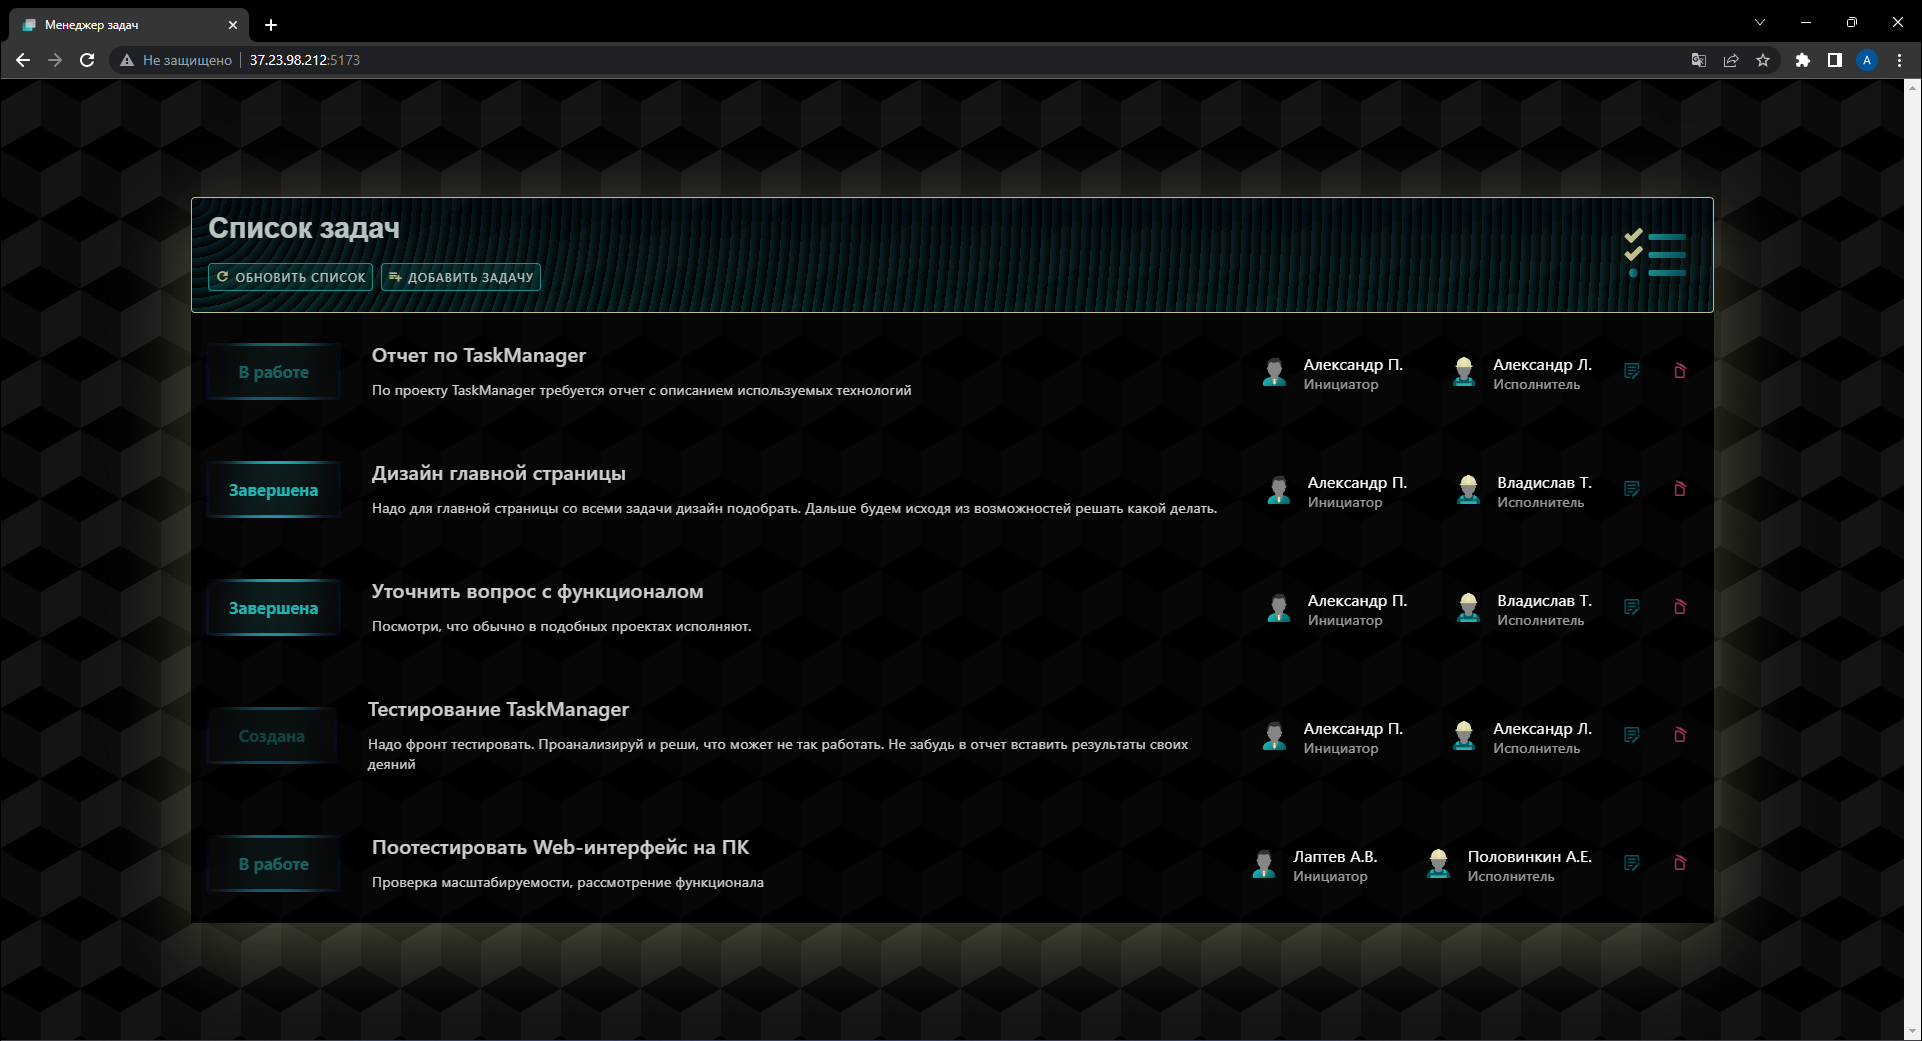
\includegraphics[scale=0.3]{main_screen.png}
    \caption{Главное окно приложения}
    \label{fig:mainscreen}
\end{figure}

\section*{Удаление (закрытие) задачи}
\addcontentsline{toc}{section}{Удаление (закрытие) задачи}

Напротив каждой задачи с правой стороны есть две кнопки, которые отвечают за редактирование задачи и удаление. Чтобы удалить задачу достаточно нажать на красную урну. Никаких подтверждений при этом не требуется, удаление происходит в одно действие.

\section*{Редактирование задачи}
\addcontentsline{toc}{section}{Редактирование задачи}

Для редактирования задачи нужно нажать соответствующую кнопку со списком (синего цвета). После этого откроется окно с задачей, в которую можно вносить изменения по всем доступным полям. Поля, доступные для редактирования:

\begin{enumerate}
    \item Название задачи

    \item Описание задачи

    \item Инициатор задачи

    \item Исполнитель задачи

    \item Статус задачи
\end{enumerate}

\begin{figure}[H]
    \centering
    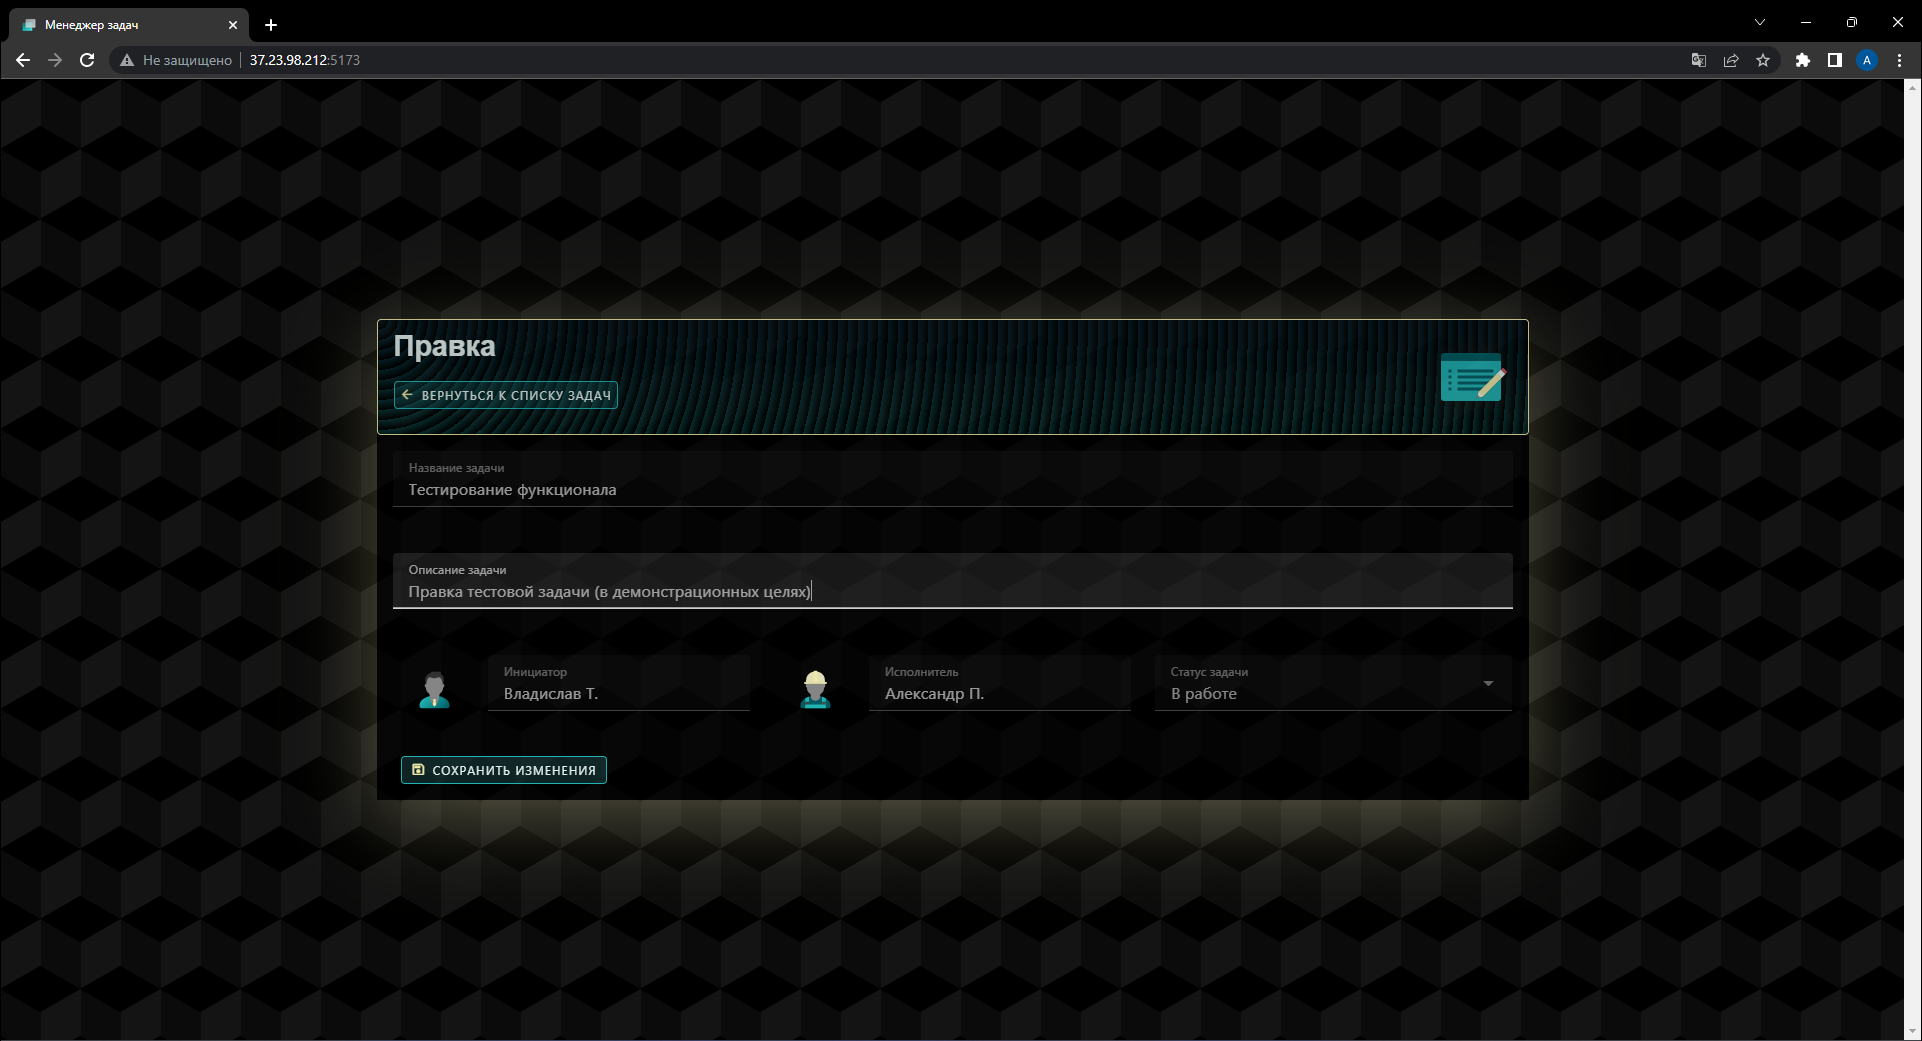
\includegraphics[scale=0.3]{edit_task.png}
    \caption{Окно для редактирования выбранной задачи}
    \label{fig:edittask}
\end{figure}

Также в окне присутствуют две кнопки: для сохранения изменений и для возврата к главной странице.

\section*{Создание новой задачи}
\addcontentsline{toc}{section}{Создание новой задачи}

Чтобы создать новую задачу нужно, как уже упоминалось, нужно нажать соответствующую кнопку в меню на главном экране. После этого появится окно, которое похоже на окно редактирования задачи. Вид этого она показан на рис. 3.

\begin{figure}[H]
    \centering
    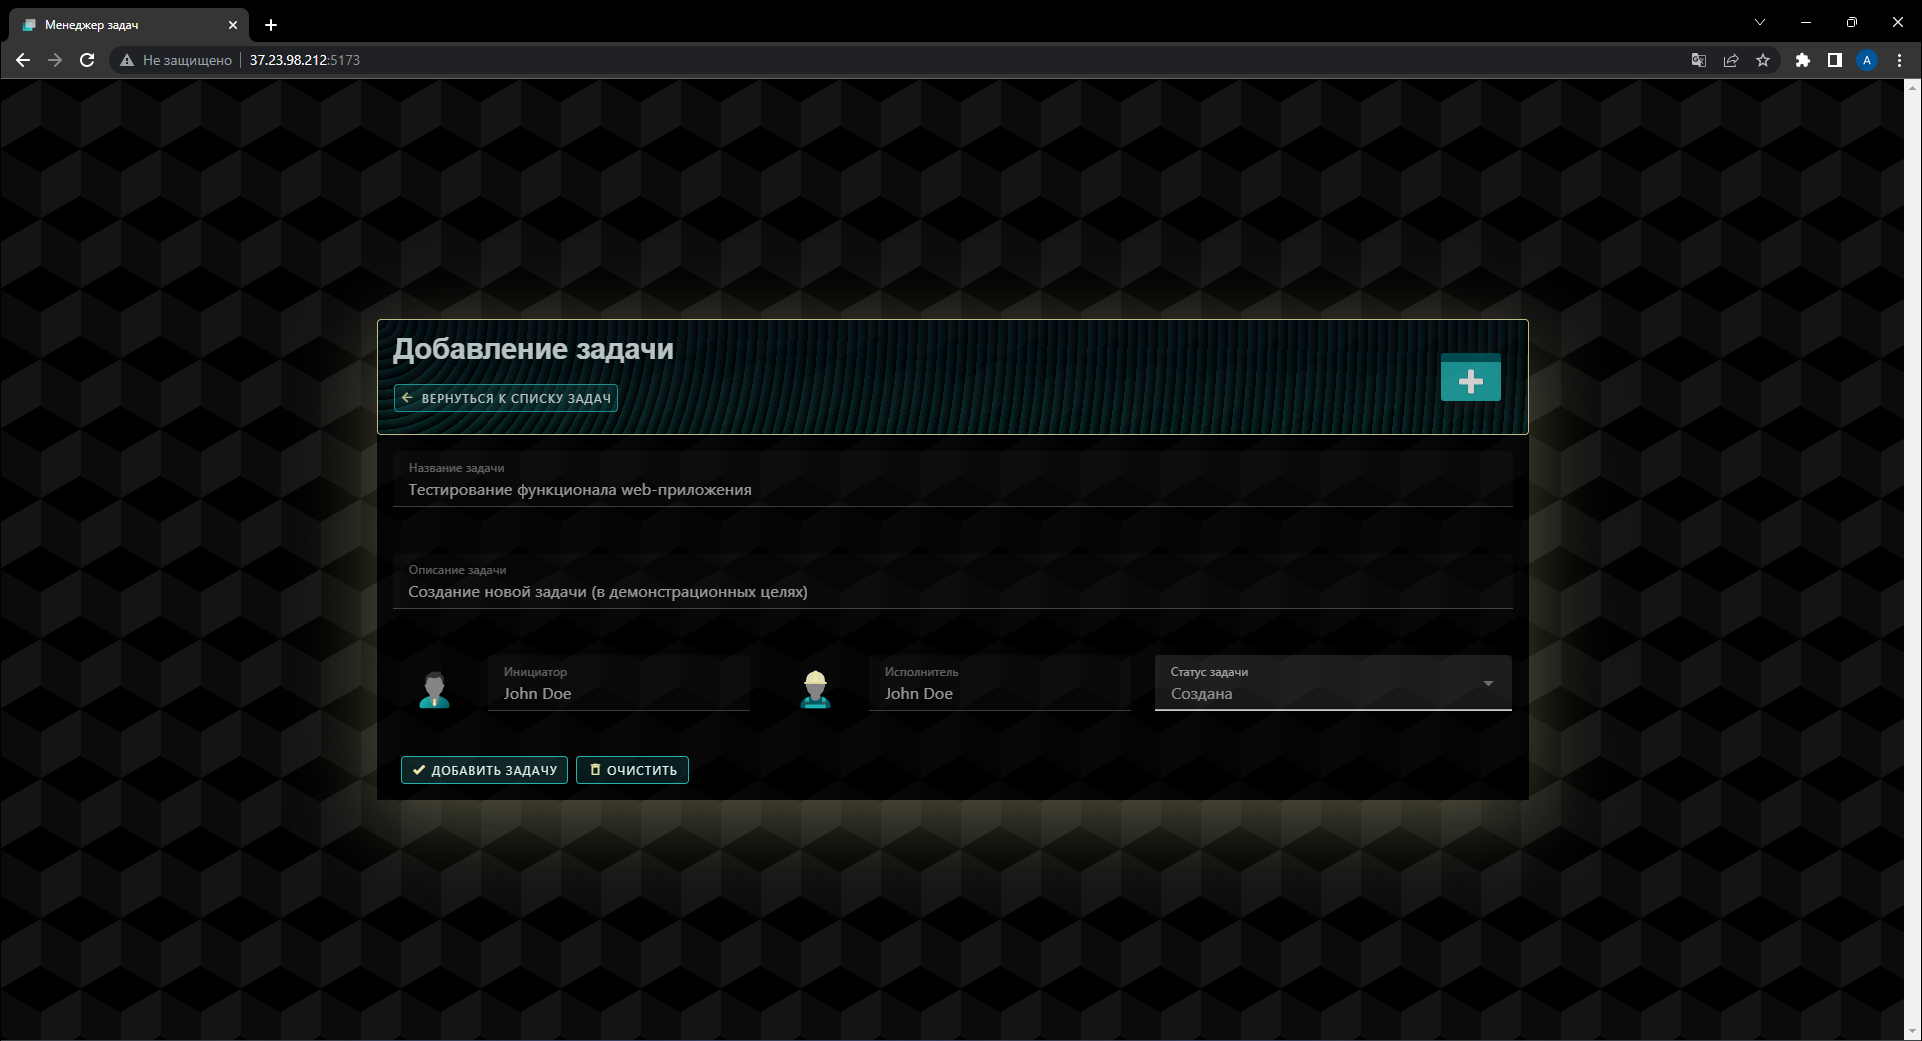
\includegraphics[scale=0.3]{add_task.png}
    \caption{Окно для создания новой задачи}
    \label{fig:addtask}
\end{figure}

Здесь также нужно заполнить те же самые поля, единственным отличием является наличие кнопки <<Очистить>>, которая очищает все введенные данные и вместо кнопки сохранения изменений появляется кнопка <<Добавить задачу>>.

% \chapter*{Приложение 1}
% \addcontentsline{toc}{chapter}{Приложение 1}

\chapter*{Приложение 2}
\addcontentsline{toc}{chapter}{Приложение 2}

\begin{code}
\captionof{listing}{Схема БД}
\label{code:pi-example}
\begin{minted}[mathescape,linenos,frame=lines,breaklines]{Python}
from sqlalchemy.schema import Column
from sqlalchemy.types import Text, JSON
from sqlalchemy.dialects.postgresql import UUID
import uuid

from app.database import Base

class Task(Base):
   __tablename__ = "Tasks"
   task_uuid = Column(UUID(as_uuid=True), primary_key=True, default=uuid.uuid4)
   task_description = Column(Text())
   task_name = Column(Text())
   task_params = Column(JSON)
\end{minted}
\end{code}

\begin{code}
\captionof{listing}{Vue}
\label{code:pi-example}
\begin{minted}[mathescape,linenos,frame=lines,breaklines]{Python}
<template>
  <v-container v-if="!AddTask && !EditTask" style="padding: 0px;">
  <v-card
      color="rgb(33 178 178)"
      theme="dark"
      variant="outlined"
  >
    <div class="d-flex flex-no-wrap justify-space-between">
      <div>
        <v-card-title class="text-h5" >
          Список задач
        </v-card-title>

<!--        <v-card-subtitle>Выберете задачу и вы сможете просмотреть, отредактировать или удалить её</v-card-subtitle>-->

        <v-card-actions v-if="!this.$vuetify.display.mobile">
          <v-btn
              class="ms-2"
              variant="outlined"
              size="small"
              v-on:click="update_task_list()"
              id = "v-btn_on_header"
          ><v-icon  id="task_on_header" >mdi-refresh</v-icon>Обновить список</v-btn>   <!--              v-on:click="update_task_list()"--> <!--              prepend-icon="mdi-refresh"-->
          <v-btn
              class="ms-2"
              variant="outlined"
              size="small"
              v-on:click="add_new_task()"
              id = "v-btn_on_header"
          ><v-icon id="task_on_header" >mdi-playlist-plus</v-icon>Добавить задачу</v-btn>
        </v-card-actions>


        <v-card-actions v-if="this.$vuetify.display.mobile">
          <v-btn
              class="ms-2"
              variant="outlined"
              size="large"
              v-on:click="update_task_list()"
              id = "v-btn_on_header"
          ><v-icon  id="task_on_header" >mdi-refresh</v-icon></v-btn>   <!--              v-on:click="update_task_list()"--> <!--              prepend-icon="mdi-refresh"-->
          <v-btn
              class="ms-2"
              variant="outlined"
              size="large"
              v-on:click="add_new_task()"
              id = "v-btn_on_header"
          ><v-icon id="task_on_header" >mdi-playlist-plus</v-icon></v-btn>
<!--          <v-btn-->
<!--              class="ms-2"-->
<!--              variant="outlined"-->
<!--              size="large"-->
<!--              id = "v-btn_on_header"-->
<!--          ><v-icon id="task_on_header" >mdi-translate-variant</v-icon></v-btn>-->
        </v-card-actions>
      </div>

      <v-avatar
          class="ma-3"
          size="6em"
          rounded="0"
      >
        <v-img id="todo_svg" src="/todo.svg"></v-img>
      </v-avatar>
    </div>
  </v-card>



<!--      <v-list lines="three">-->
<!--      <v-list-item-->
<!--          v-for="task in TasksArray"-->
<!--          v-on:click="select_task(task['task_uuid'])"-->
<!--          :key="task['task_name']"-->
<!--          :title="task['task_name']"-->
<!--          :subtitle="task['task_description']"> &lt;!&ndash;  append-icon="mdi-delete-empty-outline"&ndash;&gt;-->
<!--        <template v-slot:prepend="{ isActive }">-->

<!--          <v-list-item__content>-->
<!--         <v-list-item-title>{{task['task_name']}}</v-list-item-title>-->
<!--          <v-list-item-subtitle>{{task['task_description']}}</v-list-item-subtitle>-->
<!--            </v-list-item__content>-->
<!--          <v-list-item-action start>-->

<!--            <v-btn stacked  append-icon="mdi-text-box-edit-outline" variant="outlined"></v-btn>-->
<!--            <v-btn stacked  append-icon="mdi-delete-empty-outline" variant="outlined"></v-btn>-->
<!--          </v-list-item-action>-->
<!--        </template>-->
<!--      </v-list-item>-->
<!--    </v-list>-->


  <v-table id="tasks_table" max-height="70vh">
  <v-toolbar
      height="20%"
      class="mb-0"
      dark
      prominent
      v-for="task in TasksArray"
  >


<!--      <div v-if="task['task_params']['task_status']==='Assigned'" class="square" id="status_Assigned">-->
<!--      </div>-->
<!--      <div v-if="task['task_params']['task_status']==='In_Process'" class="square" id="status_In_Process">-->
<!--      </div>-->
<!--      <div v-if="task['task_params']['task_status']==='Finalized'" class="square" id="status_Finalized">-->
<!--      </div>-->
<!--      <div v-if="task['task_params']['task_status']==='Closed'" class="square" id="status_Closed">-->
<!--      </div>-->
    <div v-if="task['task_params']['task_status']==='Assigned' && !this.$vuetify.display.mobile" class="card" id="Assigned">
      <h2>Создана</h2>
    </div>
    <div v-if="task['task_params']['task_status']==='In_Process' && !this.$vuetify.display.mobile" class="card" id="In_Process">
      <h2>В работе</h2>
    </div>
    <div v-if="task['task_params']['task_status']==='Finalized' && !this.$vuetify.display.mobile" class="card" id="Finalized">
      <h2>Завершается</h2>
    </div>
    <div v-if="task['task_params']['task_status']==='Closed' && !this.$vuetify.display.mobile" class="card" id="Closed">
      <h2>Завершена</h2>
    </div>

    <v-card
        :title="task['task_name']"
        :text="task['task_description']"
        id="toc"
    ><div class="square"></div></v-card>
    <v-spacer></v-spacer>

<!--    <v-card-->
<!--        :subtitle="task['task_params']['task_status']"-->
<!--        style="min-width: 9vw; max-width: 9vw; background-color: #009E73"-->
<!--    ></v-card>-->



<!--    <v-card-->
<!--        class="mx-auto"-->
<!--        style="background-image: none; background-color: transparent"-->
<!--    >-->
<!--      <template v-slot:prepend>-->
<!--        <v-avatar-->
<!--            class="ma-3"-->
<!--            size="2.3em"-->
<!--            rounded="0"-->
<!--        >-->
<!--          <v-img src="/init.svg"></v-img>-->
<!--        </v-avatar>-->
<!--      </template>-->
<!--    </v-card>-->

    <v-list-item
        v-if="!this.$vuetify.display.mobile"
        :title="task['task_params']['task_initiator']"
        :subtitle="'Инициатор'"
        class="pa-2 ma-2"
        >
      <template v-slot:prepend>
        <v-avatar
            class="ma-3"
            size="2.3em"
            rounded="0"
        >
          <v-img src="/init.svg"></v-img>
        </v-avatar>
      </template>
    </v-list-item>

    <v-list-item
        v-if="!this.$vuetify.display.mobile"
        :title="task['task_params']['task_executor']"
        :subtitle="'Исполнитель'"
        class="pa-2 ma-2"
        >
            <template v-slot:prepend>
              <v-avatar
                  class="ma-3"
                  size="2.3em"
                  rounded="0"
              >
                <v-img src="/exec.svg"></v-img>
              </v-avatar>
            </template>
    </v-list-item>


    <v-btn icon id="btn-card-task-edit" v-on:click="edit_task(task)">
      <v-icon>mdi-text-box-edit-outline</v-icon>
    </v-btn>
    <v-btn icon id="btn-card-task-delete" v-on:click="delete_task(task['task_uuid'])">
      <v-icon>mdi-delete-empty-outline</v-icon>
    </v-btn>
  </v-toolbar>
  </v-table>
  </v-container>

  <v-container v-if="AddTask" id="container_add_Task" style="padding: 0px;" >
    <v-card
        color="rgb(33 178 178)"
        theme="dark"
        variant="outlined"
    >
      <div class="d-flex flex-no-wrap justify-space-between">
        <div>
          <v-card-title v-if="!this.$vuetify.display.mobile" class="text-h5" >
            Добавление задачи
          </v-card-title>
          <v-card-title v-if="this.$vuetify.display.mobile" class="text-h5" >
            Добавление
          </v-card-title>
          <v-card-actions>
            <v-btn
                v-if="!this.$vuetify.display.mobile"
                class="ms-2"
                variant="outlined"
                size="small"
                v-on:click="add_new_task()"
                id = "v-btn_on_header"
            ><v-icon id="task_on_header" >mdi-arrow-left</v-icon>Вернуться к списку задач</v-btn>
            <v-btn
                v-if="this.$vuetify.display.mobile"
                class="ms-2"
                variant="outlined"
                size="small"
                v-on:click="add_new_task()"
                id = "v-btn_on_header"
            ><v-icon id="task_on_header" >mdi-arrow-left</v-icon>К списку задач</v-btn>
          </v-card-actions>
        </div>
        <v-avatar
            class="ma-3"
            size="6em"
            rounded="0"
        >
          <v-img id="todo_svg" src="/add_task.svg"></v-img>
        </v-avatar>
      </div>
    </v-card>

    <v-form>
      <v-container>
        <v-row>
          <v-col
              cols="12"
              md="12"
          >
            <v-text-field
                v-model="task_name"
                :rules="nameRules"
                :counter="10"
                label="Название задачи"
                required
            ></v-text-field>
          </v-col>
        </v-row>

        <v-row>
          <v-col
              cols="12"
              md="12"
          >
            <v-text-field
                v-model="task_description"
                :rules="nameRules"
                :counter="10"
                label="Описание задачи"
                required
            ></v-text-field>
          </v-col>
        </v-row>

        <v-row>
          <v-col
              cols="12"
              md="1"
              style="text-align: center; padding-right: 0px;"
          >
            <v-avatar
                class="ma-3"
                size="3em"
                rounded="0"
            >
              <v-img src="/init.svg"></v-img>
            </v-avatar>
          </v-col>
          <v-col
              cols="12"
              md="3"
          >
            <v-text-field
                v-model="task_initiator"
                :rules="nameRules"
                :counter="10"
                label="Инициатор"
                required
            ></v-text-field>
          </v-col>


          <v-col
              cols="12"
              md="1"
              style="text-align: center; padding-right: 0px;"
          >
            <v-avatar
                class="ma-3"
                size="3em"
                rounded="0"
            >
              <v-img src="/exec.svg"></v-img>
            </v-avatar>
          </v-col>
          <v-col
              cols="12"
              md="3"
          >

            <v-text-field
                v-model="task_executor"
                :rules="nameRules"
                :counter="10"
                label="Исполнитель"
                required
            ></v-text-field>
          </v-col>

          <v-col
              cols="12"
              md="4"
          >
<!--            "['Assigned', 'In_Process', 'Finalized', 'Closed' ]"-->
            <v-select
                v-model="task_status"
                :items="['Создана', 'В работе', 'Завершается', 'Завершена' ]"
                label="Статус задачи"
            ></v-select>
          </v-col>

        </v-row>
        <v-btn
            class="ms-2"
            variant="outlined"
            size="small"
            v-on:click="create_new_task()"
            id = "v-btn_on_header"
        ><v-icon id="task_on_header" >mdi-check-bold</v-icon>Добавить задачу</v-btn>
        <v-btn
            class="ms-2"
            variant="outlined"
            size="small"
            v-on:click="clear_task_params()"
            id = "v-btn_on_header"
        ><v-icon id="task_on_header" >mdi-delete-outline</v-icon>Очистить</v-btn>
      </v-container>

    </v-form>

  </v-container>

  <v-container v-if="EditTask" id="container_add_Task" style="padding: 0px;" >
    <v-card
        color="rgb(33 178 178)"
        theme="dark"
        variant="outlined"
    >
      <div class="d-flex flex-no-wrap justify-space-between">
        <div>
          <v-card-title class="text-h5" >
            Правка
          </v-card-title>
          <v-card-actions>
            <v-btn
                v-if="!this.$vuetify.display.mobile"
                class="ms-2"
                variant="outlined"
                size="small"
                v-on:click="show_edit_task()"
                id = "v-btn_on_header"
            ><v-icon id="task_on_header" >mdi-arrow-left</v-icon>Вернуться к списку задач</v-btn>
            <v-btn
                v-if="this.$vuetify.display.mobile"
                class="ms-2"
                variant="outlined"
                size="small"
                v-on:click="show_edit_task()"
                id = "v-btn_on_header"
            ><v-icon id="task_on_header" >mdi-arrow-left</v-icon>К списку задач</v-btn>
          </v-card-actions>
        </div>
        <v-avatar
            class="ma-3"
            size="6em"
            rounded="0"
        >
          <v-img id="todo_svg" src="/edit.svg"></v-img>
        </v-avatar>
      </div>
    </v-card>

    <v-form>
      <v-container>
        <v-row>
          <v-col
              cols="12"
              md="12"
          >
            <v-text-field
                v-model="task_name"
                :rules="nameRules"
                :counter="10"
                label="Название задачи"
                required
            ></v-text-field>
          </v-col>
        </v-row>

        <v-row>
          <v-col
              cols="12"
              md="12"
          >
            <v-text-field
                v-model="task_description"
                :rules="nameRules"
                :counter="10"
                label="Описание задачи"
                required
            ></v-text-field>
          </v-col>
        </v-row>

        <v-row>
          <v-col
              cols="12"
              md="1"
              style="text-align: center; padding-right: 0px;"
          >
            <v-avatar
                class="ma-3"
                size="3em"
                rounded="0"
            >
              <v-img src="/init.svg"></v-img>
            </v-avatar>
          </v-col>
          <v-col
              cols="12"
              md="3"
          >
            <v-text-field
                v-model="task_initiator"
                :rules="nameRules"
                :counter="10"
                label="Инициатор"
                required
            ></v-text-field>
          </v-col>


          <v-col
              cols="12"
              md="1"
              style="text-align: center; padding-right: 0px;"
          >
            <v-avatar
                class="ma-3"
                size="3em"
                rounded="0"
            >
              <v-img src="/exec.svg"></v-img>
            </v-avatar>
          </v-col>
          <v-col
              cols="12"
              md="3"
          >

            <v-text-field
                v-model="task_executor"
                :rules="nameRules"
                :counter="10"
                label="Исполнитель"
                required
            ></v-text-field>
          </v-col>

          <v-col
              cols="12"
              md="4"
          >
            <!--            "['Assigned', 'In_Process', 'Finalized', 'Closed' ]"-->
            <v-select
                v-model="task_status"
                :items="['Создана', 'В работе', 'Завершается', 'Завершена' ]"
                label="Статус задачи"
            ></v-select>
          </v-col>

        </v-row>
        <v-btn
            class="ms-2"
            variant="outlined"
            size="small"
            v-on:click="update_task()"
            id = "v-btn_on_header"
        ><v-icon id="task_on_header" >mdi-content-save-outline</v-icon>Сохранить изменения</v-btn>
      </v-container>

    </v-form>

  </v-container>
</template>

<script>
import axios from 'axios'
export default {
  name: "TaskList",
  data() {
    return {
      TasksArray: [],
      AddTask: false,
      task_name: "",
      task_description: "",
      task_initiator: "",
      task_executor: "",
      task_status: "",
      task_uuid: "",
      EditTask: false,
    }
  },
  mounted() {
    console.log(this.$vuetify.display.mobile)
    axios({
      method: "get",
      url: `/api/tasks`,
    })
        .then(response => {
          console.log(response.data);
          // console.log(response);
          this.TasksArray = response.data;
        });
    // fetch("/api/tasks")
    //     .then((response) =>response.json())
    //     .then((json) => {
    //           console.log(json)});
  },
  methods: {
    show_edit_task() {
      this.update_task_list()
      this.EditTask = !this.EditTask
    },
    edit_task(selected_task) {
      console.log(" ")
      console.log("Edit")
      console.log(selected_task)
      this.task_name = selected_task['task_name']
      this.task_description = selected_task['task_description']
      this.task_executor = selected_task['task_params']['task_executor']
      this.task_initiator = selected_task['task_params']['task_initiator']
      this.task_uuid = selected_task['task_uuid']
      if (selected_task['task_params']['task_status']==='Assigned') {
        this.task_status ='Создана'
        // "['Assigned', 'In_Process', 'Finalized', 'Closed' ]"
        // "['Создана', 'В работе', 'Завершается', 'Завершена' ]"
      }
      else if  (selected_task['task_params']['task_status']==='In_Process') {
        this.task_status ='В работе'
      }
      else if  (selected_task['task_params']['task_status']==='Finalized') {
        this.task_status ='Завершается'
      }
      else if  (selected_task['task_params']['task_status'] ==='Closed') {
        this.task_status ='Завершена'
      }
      else {
        this.task_status ='Создана'
      }
      this.show_edit_task()
      // this.$emit('pointselected', point_name);
      // this.$router.replace({ name: "SettingUp" });
    },
    update_task() {
      let task_status_real
      if (this.task_status==='Создана') {
        task_status_real = 'Assigned'
        // "['Assigned', 'In_Process', 'Finalized', 'Closed' ]"
        // "['Создана', 'В работе', 'Завершается', 'Завершена' ]"
      }
      else if  (this.task_status==='В работе') {
        task_status_real = 'In_Process'
      }
      else if  (this.task_status==='Завершается') {
        task_status_real = 'Finalized'
      }
      else if  (this.task_status==='Завершена') {
        task_status_real = 'Closed'
      }
      else {
        task_status_real = 'Assigned'
      }
      axios.put('/api/tasks/'+this.task_uuid, {
        task_name: this.task_name,
        task_description: this.task_description,
        task_params: {
          task_initiator: this.task_initiator,
          task_executor: this.task_executor,
          task_status: task_status_real,
        }
      })
          .then((response) => {
            console.log(response);
            this.show_edit_task()
          }, (error) => {
            console.log(error);
          });
    },
    delete_task(selected_task_uuid) {
      console.log(" ")
      console.log("Delete")
      console.log(selected_task_uuid)
      axios({
        method: "delete",
        url: `/api/tasks/`+selected_task_uuid,
      })
          .then(response => {
            axios({
              method: "get",
              url: `/api/tasks`,
            })
                .then(response => {
                  this.TasksArray = response.data;
                });
          });
    },
    update_task_list() {
      axios({
        method: "get",
        url: `/api/tasks`,
      })
          .then(response => {
            console.log(response.data);
            this.TasksArray = response.data;
          });
    },
    clear_task_params (){
      this.task_name = "";
      this.task_description = "";
      this.task_initiator= "";
      this.task_executor = "";
      this.task_status = "";
    },
    add_new_task() {
      this.update_task_list()
      this.AddTask = !this.AddTask
      this.clear_task_params()
      console.log(" ")
      console.log("Add")
    },
    create_new_task() {
      let task_status_real
      if (this.task_status==='Создана') {
        task_status_real = 'Assigned'
        // "['Assigned', 'In_Process', 'Finalized', 'Closed' ]"
        // "['Создана', 'В работе', 'Завершается', 'Завершена' ]"
      }
      else if  (this.task_status==='В работе') {
        task_status_real = 'In_Process'
      }
      else if  (this.task_status==='Завершается') {
        task_status_real = 'Finalized'
      }
      else if  (this.task_status==='Завершена') {
        task_status_real = 'Closed'
      }
      else {
        task_status_real = 'Assigned'
      }
      axios.post('/api/tasks/add', {
        task_name: this.task_name,
        task_description: this.task_description,
        task_params: {
          task_initiator: this.task_initiator,
          task_executor: this.task_executor,
          task_status: task_status_real,
        }
      })
          .then((response) => {
            console.log(response);
            this.add_new_task()
          }, (error) => {
            console.log(error);
          });
    }
  }
}
</script>
<style scoped>

#container_add_Task{
  min-width: 60vw;
  margin: 0px;
}
#tasks_table {
  background: transparent;
}
#status_Assigned {
  height: 100%;
  width: calc(3vw);
  background-color: #21B2B2;
}
#status_In_Process {
  height: 100%;
  width: 3%;
  background-color: #009E73;
}
#status_Finalized {
  height: 100%;
  width: 3%;
  background-color: #06614C;
}
#status_Closed {
  height: 100%;
  width: 3%;
  background-color: #182C25;
}

.v-card {
  /*box-shadow: rgb(192 187 137 / 60%) 0px 30px 60px -12px, rgb(194 189 139 / 37%) 0px 18px 36px -18px;*/
  /*box-shadow: rgba(238, 232, 169, 0.33) 0px 20px 80px;*/
  border-color: #EEE8A9;
  background-color: #000000;
  opacity: 0.8;
  background-image:  repeating-radial-gradient( circle at 0 0, transparent 0, #000000 10px ), repeating-linear-gradient( rgba(33, 178, 247, 0.15), rgba(33, 178, 178, 0.3));
}

button{
  margin-top: 2%;
}

.v-btn {
  color: #e6f4f1;
  border-color: #21B2B2;
}

.v-card .v-card-title  {
  padding-top: 4%;
  color: #e6f4f1;
  font-size: 1.8rem !important;
  font-weight: bold !important;
  /*font-size: calc(0.002vw + 0.002vh + 1.5vmin);*/
}
.v-card .v-card-subtitle{
  color: #e6f4f1;
  font-size: 1rem !important;
}

.v-card-item__content .v-card-title  {
}

.v-toolbar {
  background: rgba(0, 0, 0, 0.63);
  color: white;
}


span .v-btn__content {
  color: #e6f4f1;
}

#toc{
  background-color: transparent;
  background-image: none;
  border-color: transparent;
  box-shadow: none;
  padding-top: 15px;
  padding-bottom: 15px;
  color: white;
}
/*#toc.v-card-title {*/
/*  font-size: 1rem !important;*/
/*}*/

#btn-card-task-edit{
  margin-top: 0%;
  /*color: #324B4B;*/
  color: #005c64;
}

#btn-card-task-delete {
  margin-top: 0%;
  color: #A73160;
}

#v-btn_on_header  {
  background-color: rgb(33 178 178 / 15%);
}

#task_on_header {
  margin-right: 3%;
  color: #EEE8A9;
}
.v-btn--icon .v-icon {
  --v-icon-size-multiplier: 0.85;
}

#todo_svg{
  /*filter: drop-shadow( 5px 5px 8px rgba(33, 178, 178, 0.37));*/
  filter: drop-shadow( 1px 1px 9px rgb(22, 22, 22));
  height: 80%;
}

.v-table__wrapper {
  max-height: calc(60vh) !important;
}

.card {
  min-width: 120px;
  width: 7vw;
  height: 6vh;
  background: transparent;
  position: relative;
  display: flex;
  place-content: center;
  place-items: center;
  overflow: hidden;
  border-radius: 0px;
  margin-right: 1%;
  margin-left: 1%;
}

#Assigned h2 {
  z-index: 1;
  color: rgba(33, 178, 178, 0.3);
  font-size: 1.1em;
  font-weight: bold;
}

#Assigned::before{
  -webkit-filter: blur(15px);
  content: '';
  position: absolute;
  width: 300px;
  /*background-image: linear-gradient(180deg, rgb(33, 178, 178), rgba(42, 169, 169, 0.8));*/
  background-image:radial-gradient(circle, rgba(33, 178, 178, 0.3), rgba(34, 179, 179, 1));
  height: 130%;
  animation: rotBGimg 6s linear infinite;
  transition: all 0.2s linear;
}

#In_Process h2 {
  z-index: 1;
  color: rgba(33, 178, 178, 0.5);
  font-size: 1.1em;
  font-weight: bold;
}

#In_Process::before{
  -webkit-filter: blur(15px);
  content: '';
  position: absolute;
  width: 300px;
  /*background-image: linear-gradient(180deg, rgb(33, 178, 178), rgba(42, 169, 169, 0.8));*/
  background-image:radial-gradient(circle, rgba(33, 178, 178, 0.5), rgba(33, 178, 178, 1));
  height: 130%;
  animation: rotBGimg 6s linear infinite;
  transition: all 0.2s linear;
}

#Finalized h2 {
  z-index: 1;
  color: rgba(33, 178, 178, 0.65);
  font-size: 1.1em;
  font-weight: bold;
}

#Finalized::before{
  -webkit-filter: blur(15px);
  content: '';
  position: absolute;
  width: 300px;
  /*background-image: linear-gradient(180deg, rgb(33, 178, 178), rgba(42, 169, 169, 0.8));*/
  background-image:radial-gradient(circle, rgba(33, 178, 178, 0.8), rgba(33, 178, 178, 1));
  height: 130%;
  animation: rotBGimg 6s linear infinite;
  transition: all 0.2s linear;
}

#Closed h2 {
  z-index: 1;
  color: rgba(33, 178, 178, 1);
  font-size: 1.1em;
  font-weight: bold;
}

#Closed::before{
  -webkit-filter: blur(15px);
  content: '';
  position: absolute;
  width: 300px;
  /*background-image: linear-gradient(180deg, rgb(33, 178, 178), rgba(42, 169, 169, 0.8));*/
  background-image:radial-gradient(circle, rgba(33, 178, 178, 1), rgba(33, 178, 178, 1));
  height: 130%;
  animation: rotBGimg 6s linear infinite;
  transition: all 0.2s linear;
}


@keyframes rotBGimg {
  from {
    transform: rotate(0deg);
  }

  to {
    transform: rotate(360deg);
  }
}

.card::after {
  content: '';
  position: absolute;
  background: rgba(9, 9, 9, 0.88);
  box-shadow: 0 8px 32px 0 rgba( 31, 38, 135, 0.37 );
  backdrop-filter: blur( 10px );
  -webkit-backdrop-filter: blur( 10px );
  border-radius: 10px;
  inset: 3px;
  border-radius: 0px;
}
/* .card:hover:before {
  background-image: linear-gradient(180deg, rgb(81, 255, 0), purple);
  animation: rotBGimg 3.5s linear infinite;
} */

.v-form {
  background: rgba(0, 0, 0, 0.63);
}


</style>
\end{minted}
\end{code}

\begin{code}
\captionof{listing}{API}
\label{code:pi-example}
\begin{minted}[mathescape,linenos,frame=lines,breaklines]{Python}
from fastapi import FastAPI, Depends, HTTPException, status
from uuid import UUID
from typing import List
from sqlalchemy.orm import Session

import app.models as models
from app.database import engine, create_session
from app.schema import TaskSchema, TaskSchemaExpanded
from app.models import Task

app = FastAPI()


@app.on_event("startup")
async def startup():
    models.Base.metadata.drop_all(bind=engine)  # await
    models.Base.metadata.create_all(bind=engine)


@app.get("/tasks", response_model=List[TaskSchemaExpanded], status_code=200)
async def read_tasks(db: Session = Depends(create_session)):
    tasks = db.query(Task).all()
    return tasks


@app.post('/tasks/add', response_model=TaskSchemaExpanded, status_code=201)
async def create_task(task: TaskSchema, db: Session = Depends(create_session)):
    new_task = Task(**task.dict())
    db.add(new_task)
    db.commit()
    return new_task


@app.put("/tasks/{task_uuid}", response_model=TaskSchemaExpanded, status_code=200)
async def update_task(task_uuid: UUID, task: TaskSchema, db: Session = Depends(create_session)):
    updating_task = db.query(Task).get(task_uuid)
    if updating_task is not None:
        updating_task.task_name = task.task_name
        updating_task.task_description = task.task_description
        updating_task.task_params = task.task_params.dict()
        # for field, value in task.task_params.dict().items():
        #     setattr(updating_task, field, value)
        db.commit()
        db.refresh(updating_task)
    else:
        raise HTTPException(status.HTTP_404_NOT_FOUND, detail="Task with UUID does not exist ")
    return updating_task


@app.delete("/tasks/{task_uuid}")
def delete_task(task_uuid: UUID, db: Session = Depends(create_session)):
    task = db.get(Task, task_uuid)
    if not task:
        raise HTTPException(status_code=404, detail="Task not found")
    db.delete(task)
    db.commit()
    return {"Task deleted successfully": True}

\end{minted}
\end{code}

\begin{code}
\captionof{listing}{Валидация данных}
\label{code:pi-example}
\begin{minted}[mathescape,linenos,frame=lines,breaklines]{Python}
from pydantic import BaseModel, Extra
from uuid import uuid4, UUID
from datetime import datetime
from typing import Literal


class TaskParamsModel(BaseModel, extra=Extra.forbid):
    task_initiator: str       # инициатор
    task_executor: str       # исполнитель
    task_status: Literal['Assigned', 'In_Process', 'Finalized', 'Closed']
    # task_deadline: datetime.date  # крайний срок
    # task_param_2:   int


class TaskSchema(BaseModel):
    task_name: str
    task_description: str
    task_params: TaskParamsModel
    class Config:
        orm_mode = True


class TaskSchemaExpanded(TaskSchema):
   task_uuid: UUID = uuid4()
   class Config:
       orm_mode = True
\end{minted}
\end{code}

\begin{code}
\captionof{listing}{Docker compose}
\label{code:pi-example}
\begin{minted}[mathescape,linenos,frame=lines,breaklines]{Python}
version: "4"
services:
  web:
    build: .
    command: bash -c 'while !</dev/tcp/db/5432; do sleep 1; done; uvicorn app.main:app --host 0.0.0.0'
    ports:
      - 8008:8000
    environment:
      - DATABASE_URL=
      postgresql://mgknn:tst@db:5432/postgres
    depends_on:
      - db
    volumes:
      - .:/app
  db:
    image: postgres:13.3
    environment:
      POSTGRES_DB: "postgres"
      POSTGRES_USER: "mgknn"
      POSTGRES_PASSWORD: "tst"
    ports:
      - "5432:5432"
    volumes:
      - postgres_data:/var/lib/postgresql/data/
volumes:
  postgres_data
\end{minted}
\end{code}

% \chapter*{Приложение 3}
% \addcontentsline{toc}{chapter}{Приложение 3}

\end{document}